\documentclass[a4paper]{article}

\usepackage[utf8]{inputenc}
\usepackage[english]{babel}
\usepackage{hyperref}
\usepackage{graphicx}
\usepackage{amsmath,amssymb,amsthm}
\usepackage{siunitx}
\usepackage{xcolor}
\usepackage{multicol}
\usepackage{caption}
\usepackage{appendix}
\usepackage{pdfpages}
\usepackage{fixltx2e}
\usepackage[version=4]{mhchem}
\usepackage{url}
\usepackage{subcaption}
\usepackage{subfig}
\usepackage[justification=centering]{caption}
\usepackage[thinc]{esdiff}
\usepackage[bottom]{footmisc}


\date{\today}
\author{Thomas Brzeski \and  Victor Dejans}
\title{Kinematic and Dynamic Analysis of a Linkage:\\ Walschaerts Valve Gear}


\begin{document}

\maketitle

\section*{Introduction}

In the context of the subject \textit{Beweging en trillingen (H01N0A)} this report treats the analysis of the linkage in a Walschaerts valve gear, a system that is used in steam locomotives. The linkage that is studied in this report is based on that in figure~\ref{fig:basistekening}.

In a first section we define all links and joints with their geometric properties in the way we used them for the assignment. We also make the motion analysis of the linkage.

Second is the kinematic analysis which finds the positions, velocities and accelerations of each bar.

The final section reports upon the inverse dynamic analysis which finds the forces and torques on the linkages' joints when a driving torque is applied to the train's wheel.



\tableofcontents
\clearpage

\section{Definition of the mechanism}

Walschaerts valve gear is a linkage that was used in steam locomotives. It connects the steam pistons and the train's wheels in a way that also regulates the steam flow.

Although in real life the pistons are the driving bodies and the wheels are the driven bodies, the assistants recommended us to analyse the mechanism in the opposite way. In this assignment, the driving torque is thus applied to the wheel instead of the pistons.

\begin{figure}[h]
	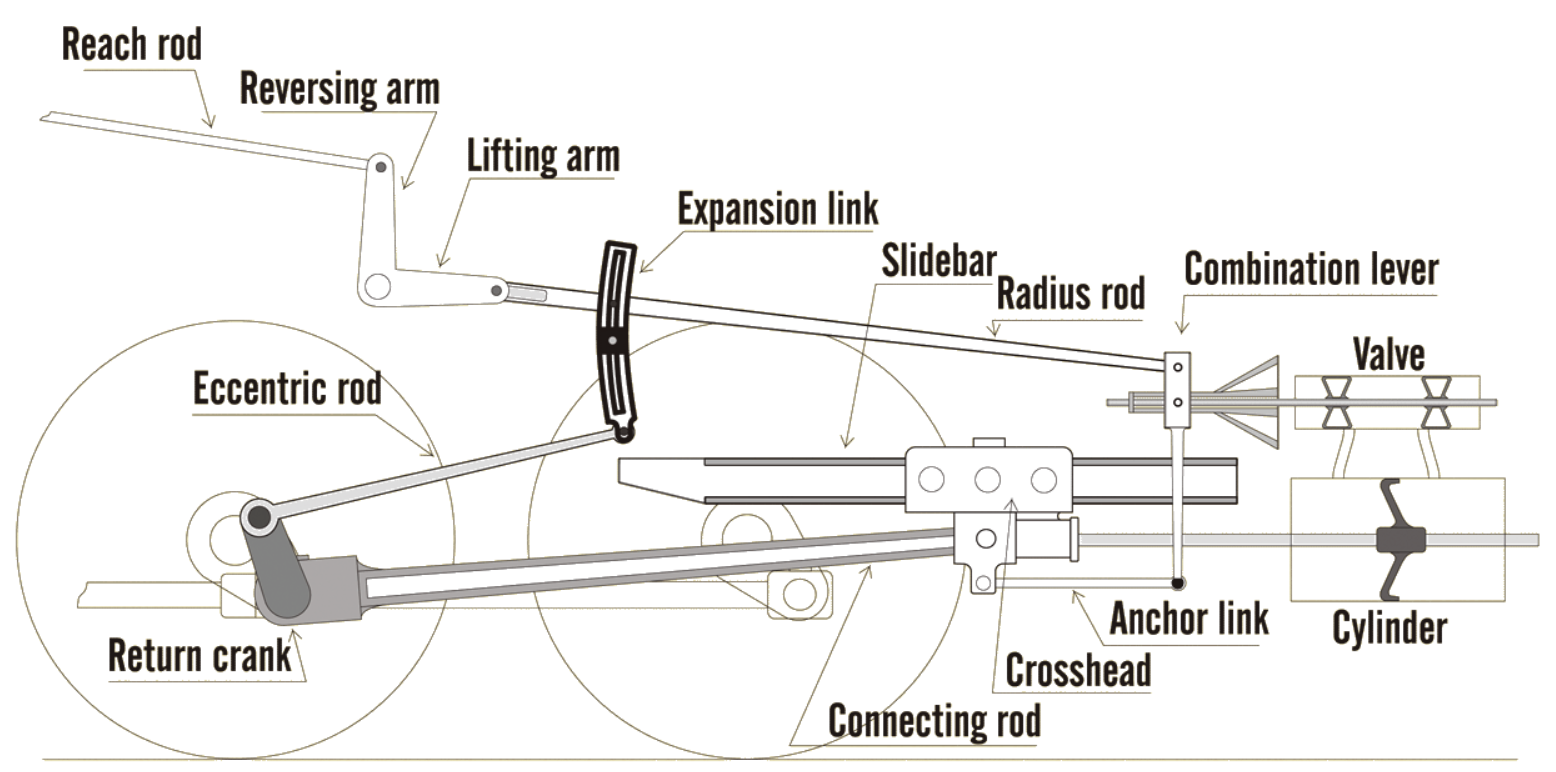
\includegraphics[width=0.9\textwidth]{wvgverslag.png}
	\centering
	\caption{Example of a Walschaerts valve gear. \cite{ove06}}
	\label{fig:basistekening}
\end{figure}

\subsection{Schematic of the mechanism and definition of the parameters}

As shown in figure~\ref{fig:schematic}, the linkage has twelve bodies.

\begin{itemize}
	\item Body \textbf{(1)} is the train. This is the ground to which other bodies are fixed.
	\item Body \textbf{(2)} is the wheel of the train. Its rotation point (A) is fixed in the origin of the xy plane. The ends of bars (3) and (12) are eccentrically attached to the wheel with hinges (B) and (C) respectively.
	\item Bodies \textbf{(3)}, \textbf{(4)}, \textbf{(7)}, \textbf{(8)}, \textbf{(10)} and \textbf{(12)} are straight bars.
	\item Body \textbf{(5)} is massless and is used to make a special joint between bar (4) and bar (7). It is attached to bar (4) with a prismatic joint (I) and to bar (7) with a hinge (H).
	\item Bar \textbf{(6)} is a kinked, L-shaped bar which consists of two parts of 95~\si{cm} long that are fixed to each other in an angle of 90~\si{degrees}. The two ends of this L-shaped bar are fixed to the ground (1) and to bar (7) with hinges.
	\item Bodies \textbf{(9)} and \textbf{(11)} are the pistons of the valve gear. Both pistons are fixed to the ground (1) with prismatic joints ((L) and (P) respectively) that only allow movement in the x direction. Their dimensions are shown in figure~\ref{fig:pistons}.
\end{itemize}

The dimensions of the bars and other bodies are defined in tables~\ref{tab:lengths} and~\ref{tab:angles}.

All bodies in this linkage are made of steel which has a density \(\rho_{steel} = 7800~\si{kg/m^3}\) \cite{steel1}.

\begin{figure}
	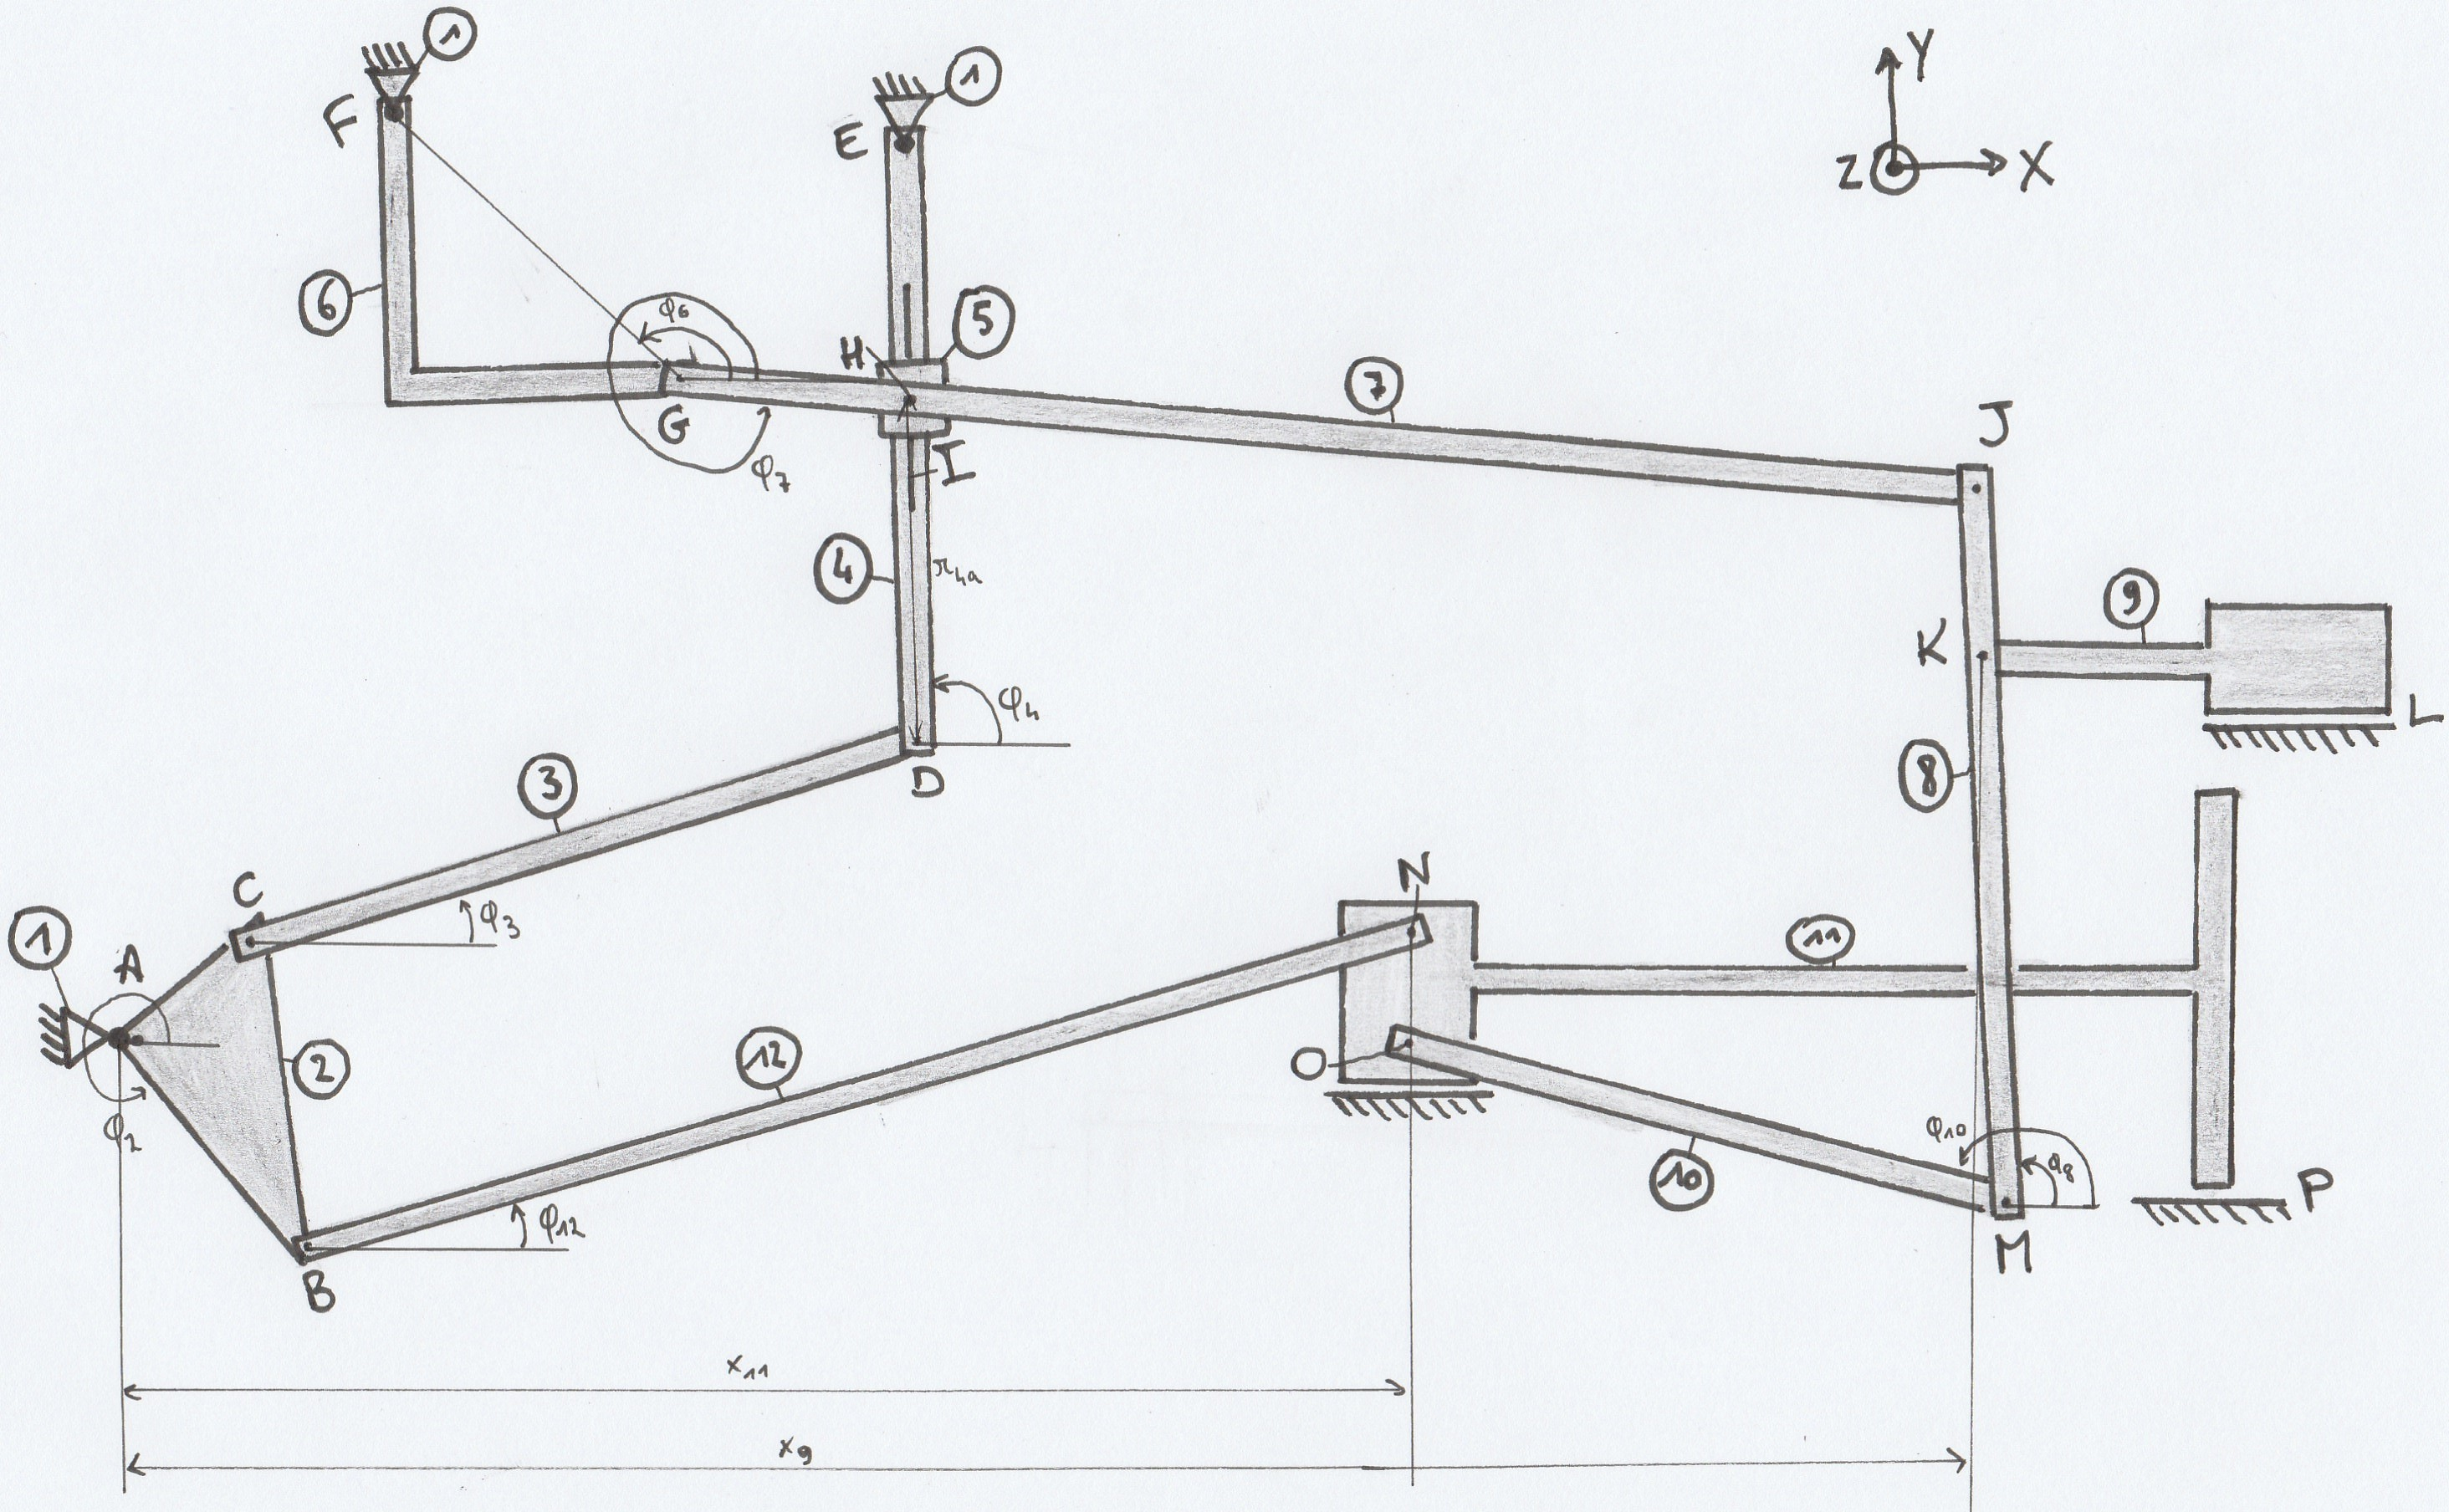
\includegraphics[width=\textwidth]{schematic.jpg}
	\centering
	\caption{Schematic representation of the studied linkage. The numbers indicate the 12 bodies. The letters indicate the 16 joints. Warning: this figure is not on scale.}
	\label{fig:schematic}
\end{figure}

\begin{table}[t]
	\centering
	\begin{tabular}{lr}
		\hline
		Bar & Length \((\si{cm})\) \\
		\hline
		1 between A and E & 321 \\
		1 between A and F & 385 \\
		2 between A and C & 27 \\
		2 between A and B & 59 \\
		3 between C and D & 299 \\
		4 between D and F & 142 \\
		6 between E and G (in a straight line) & 135 \\
		7 between G and H & 100 \\
		7 between H and J & 452 \\
		8 between J and K & 30 \\
		8 between K and M & 146 \\
		10 between O and M & 158 \\
		12 between B and N & 559 \\
		Y-coordinate of joint K \footnotemark & \\
		Y-coordinate of joint N \footnotemark & \\
		\hline
	\end{tabular}
	\footnotetext{Because}
	\caption{Lenghts of the bars and the wheel. Bars' numbers and joints' letters as indicated in figure~\ref{fig:schematic}.}
	\label{tab:lengths}
\end{table}

\begin{table} 
	\centering
	\begin{tabular}{lr}
		\hline
		Line segment & Angle to the positive x axis \((\si{degrees})\) \\
		\hline
		[AE] & 69 \\
		\text{[AF]} & 37,0188 \\
		\hline
	\end{tabular}
	\caption{Unvariable angles in the linkage's ground. Joints' letters as indicated in figure~\ref{fig:schematic}. Variable angles are calculated in section \ref{sec:kin}.}
	\label{tab:angles}
\end{table}


\begin{figure}[b]
	\centering
	
	\begin{subfigure}[b]{.4\textwidth}
		\centering
		\label{fig:piston9}
		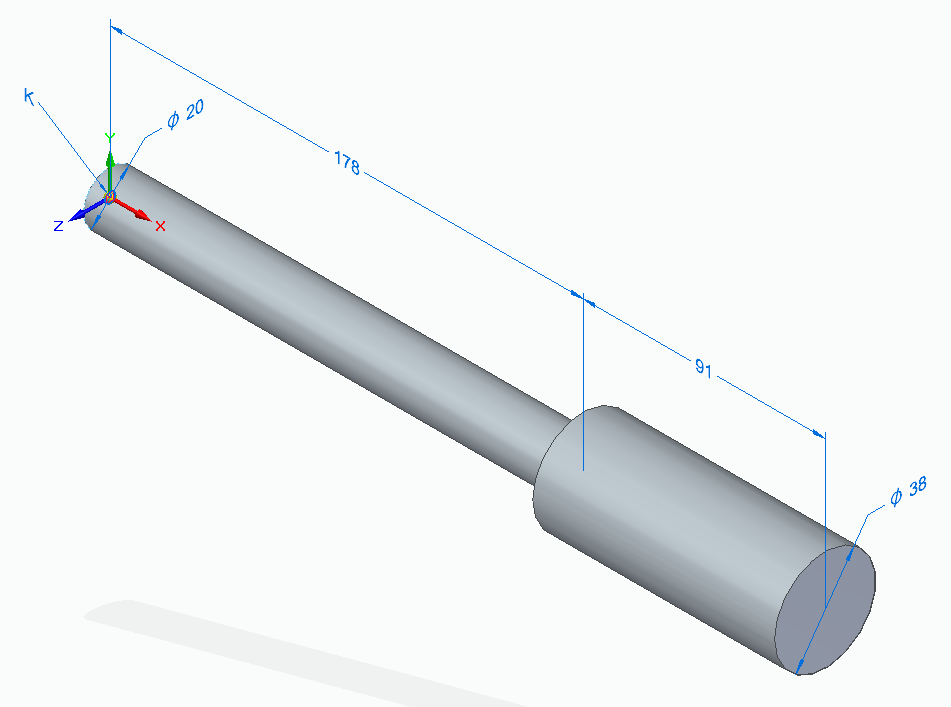
\includegraphics[width=\textwidth]{piston9.png}
		\caption{Piston (9).\centering}
	\end{subfigure}
	\hfill
	\begin{subfigure}[b]{.4\textwidth}
		\centering
		\label{fig:piston11}
		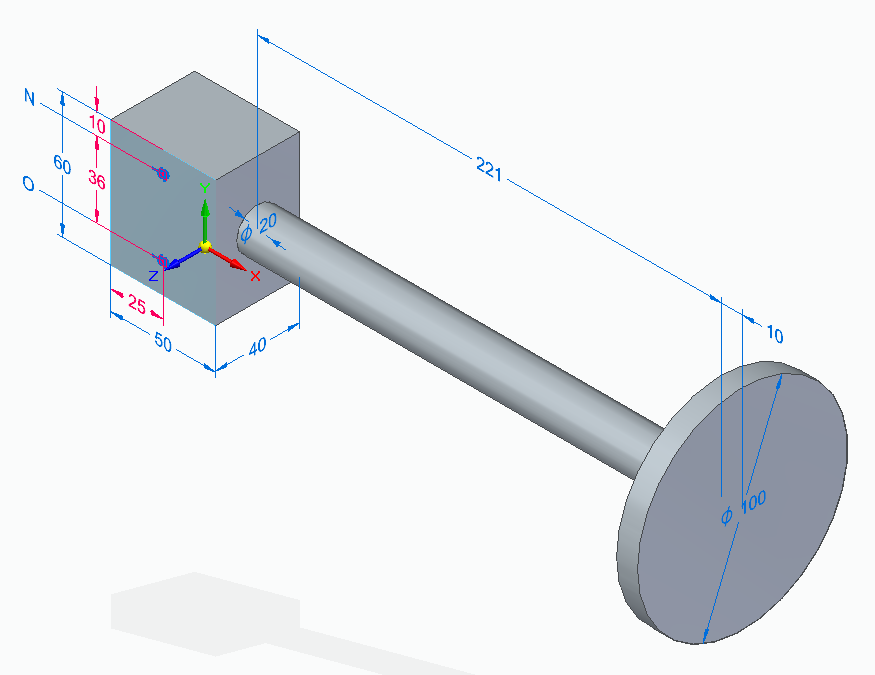
\includegraphics[width=\textwidth]{piston11.png}
		\caption{Piston (11).\centering}
	\end{subfigure}

	\caption{Pistons (9) and (11) with their dimensions in cm and with their joints with other bodies.}
	\label{fig:pistons}
	
\end{figure}



\subsection{Motion analysis}

The Walschaerts valve gear is a twelve bar linkage system with sixteen joints. This makes the mobility \(M=3*(12-1)-16*2=1\). This means the system has one degree of freedom.


\section{Kinematic analysis}
\label{sec:kin}

In the kinematic analysis we apply a driving torque to the train's wheel (body (2)) and see how the other bars react. 

The driving torque is applied to body (2) in point (A) and makes it turn with a constant angular velocity as defined in equation~\ref{eq:dphi2}, where \(\phi_2(t)\) is the angle that section [AB] of the wheel makes with the positive x axis.

\begin{equation}
	\phi_2(t) = (\pi*t)~rad \\
	\label{eq:phi2}
\end{equation}
\begin{equation}
	\diff{\phi_2(t)}{t} = \pi~rad/s \\
	\label{eq:dphi2}
\end{equation}
\begin{equation}
	\diff[2]{\phi_2(t)}{t} = 0~rad/s^2\\
\end{equation}

The kinematic analysis looks for the positions, velocities and accelerations of the other bodies in the linkage. The ten unknowns are \(\phi_3(t)\), \(\phi_4(t)\), \(r_{4a}(t)\) (the length of the part of bar (4) between joint (D) and joint (I)), \(\phi_6(t)\), \(\phi_7(t)\), \(\phi_8(t)\), \(x_9(t)\) (the x coordinate of joint (K)), \(\phi_{10}(t)\), \(x_{11}(t)\) (the x coordinate of joint (N)) and \(\phi_{12}(t)\) and their first and second order derivatives. These variables are defined in figure~\ref{fig:schematic}.

The analysis is done for 201 time samples of 0,05~seconds each.

\subsection{Position analysis}

In order to find the ten unknown positions, a set of ten "loop closure equations" is solved for each time step. A loop closure equation is the sum of all x or y vector components of linkage bodies that form a closed loop. These sums are all equal to zero. This results in a set of ten equations which are listed below in vector form \footnote{These five vector equations define the ten needed equations. Each vector can be split in one x component and one y component.}.


\begin{subequations}
\begin{equation}
	\vec{AC}+\vec{CD}+\vec{DF}-\vec{AF}=0
\end{equation}

\begin{equation}
	-\vec{GE}+\vec{GJ}-\vec{MJ}-\vec{OM}-\vec{NO}-\vec{BN}-\vec{AB}+\vec{AE}=0
\end{equation}

\begin{equation}
	\vec{AC}+\vec{CD}+\vec{DI}-\vec{GH}+\vec{GE}-\vec{AE}=0
\end{equation}

\begin{equation}
	\vec{AC}+\vec{CD}+\vec{DI}+\vec{HJ}-\vec{KJ}-\vec{AK}=0
\end{equation}

\begin{equation}
	\vec{AB}+\vec{BN}-\vec{AN}=0
\end{equation}

\label{eq:loopclosurevec}
\end{subequations}

%	\begin{subequations}
%		\begin{equation}
%		r2c*cos(\phi_2+\phi_A)+r3*cos(\phi_3)+r4*cos(\phi_4)-r1b*cos(\phi_AF)=0
%	\end{equation}
%	
%	\begin{equation}
%	r2c*sin(\phi_2+\phi_A)+r3*sin(\phi_3)+r4*sin(\phi_4)-r1b*sin(\phi_AF)=0
%	\end{equation}
%	\begin{equation}
%	%van knoop E naar knoop A langs driehoek8 en terug
%		-r6*cos(\phi_6)+r7*cos(\phi_7)-r8*cos(\phi_8)-r10*cos(\phi_10)-r11*cos(\phi_11)-r12*cos(\phi_12)-r2b*cos(\phi_2)+r1a*cos(\phi_AE)=0
%	\end{equation}
%	\begin{equation}
%	-r6*sin(\phi_6)+r7*sin(\phi_7)-r8*sin(\phi_8)-r10*sin(\phi_10)-r11*cos(\phi_11)-r12*sin(\phi_12)-r2b*sin(\phi_2)+r1a*sin(\phi_AE)=0
%	\end{equation}
%	\begin{equation}
%	%van knoop A naar knoop E langs bar3 en terug
%		r2c*cos(\phi_2+\phi_A)+r3*cos(\phi_3)+r4a*cos(\phi_4)-r7a*cos(\phi_7)+r6*cos(\phi_6)-r1a*cos(\phi_AE)=0
%	\end{equation}
%	\begin{equation}	r2c*sin(\phi_2+\phi_A)+r3*sin(\phi_3)+r4a*sin(\phi_4)-r7a*sin(\phi_7)+r6*sin(\phi_6)-r1a*sin(\phi_AE)=0
%	\end{equation}
%	\begin{equation}
%	%van knoop A naar prisma 9 en terug
%		r2c*cos(\phi_2+\phi_A)+r3*cos(\phi_3)+r4a*cos(\phi_4)+r7b*cos(\phi_7)-r8a*cos(\phi_8)-x9=0
%	\end{equation}
%	\begin{equation}
%	r2c*sin(\phi_2+\phi_A)+r3*sin(\phi_3)+r4a*sin(\phi_4)+r7b*sin(\phi_7)-r8a*sin(\phi_8)-y9=0
%	\end{equation}
%	\begin{equation}
%	%van knoop A naar prisma 11 langs bar12 en terug
%		r2b*cos(\phi_2)+r12*cos(\phi_12)-x11=0
%	\end{equation}
%	\begin{equation}
%	r2b*sin(\phi_2)+r12*sin(\phi_12)-y11=0
%	\end{equation}
%	\end{subequations}

The MATLAB function \texttt{loop\char`_closure\char`_eqs.m} lists all loop closure equations. In this case, we get a nonlinear system of equations because of the multiplication of the unknown variables \(\phi_4(t)\) and \(r_{4a}(t)\). The MATLAB function \texttt{fsolve} is used to solve this nonlinear set.

After solving this system for each of the 201 time samples, the MATLAB code returns values for each of the ten unknowns in function of the time. The plots of these ten variables are shown in figure~\ref{fig:kinpos}.

\begin{figure}[h]
	\centering
	
	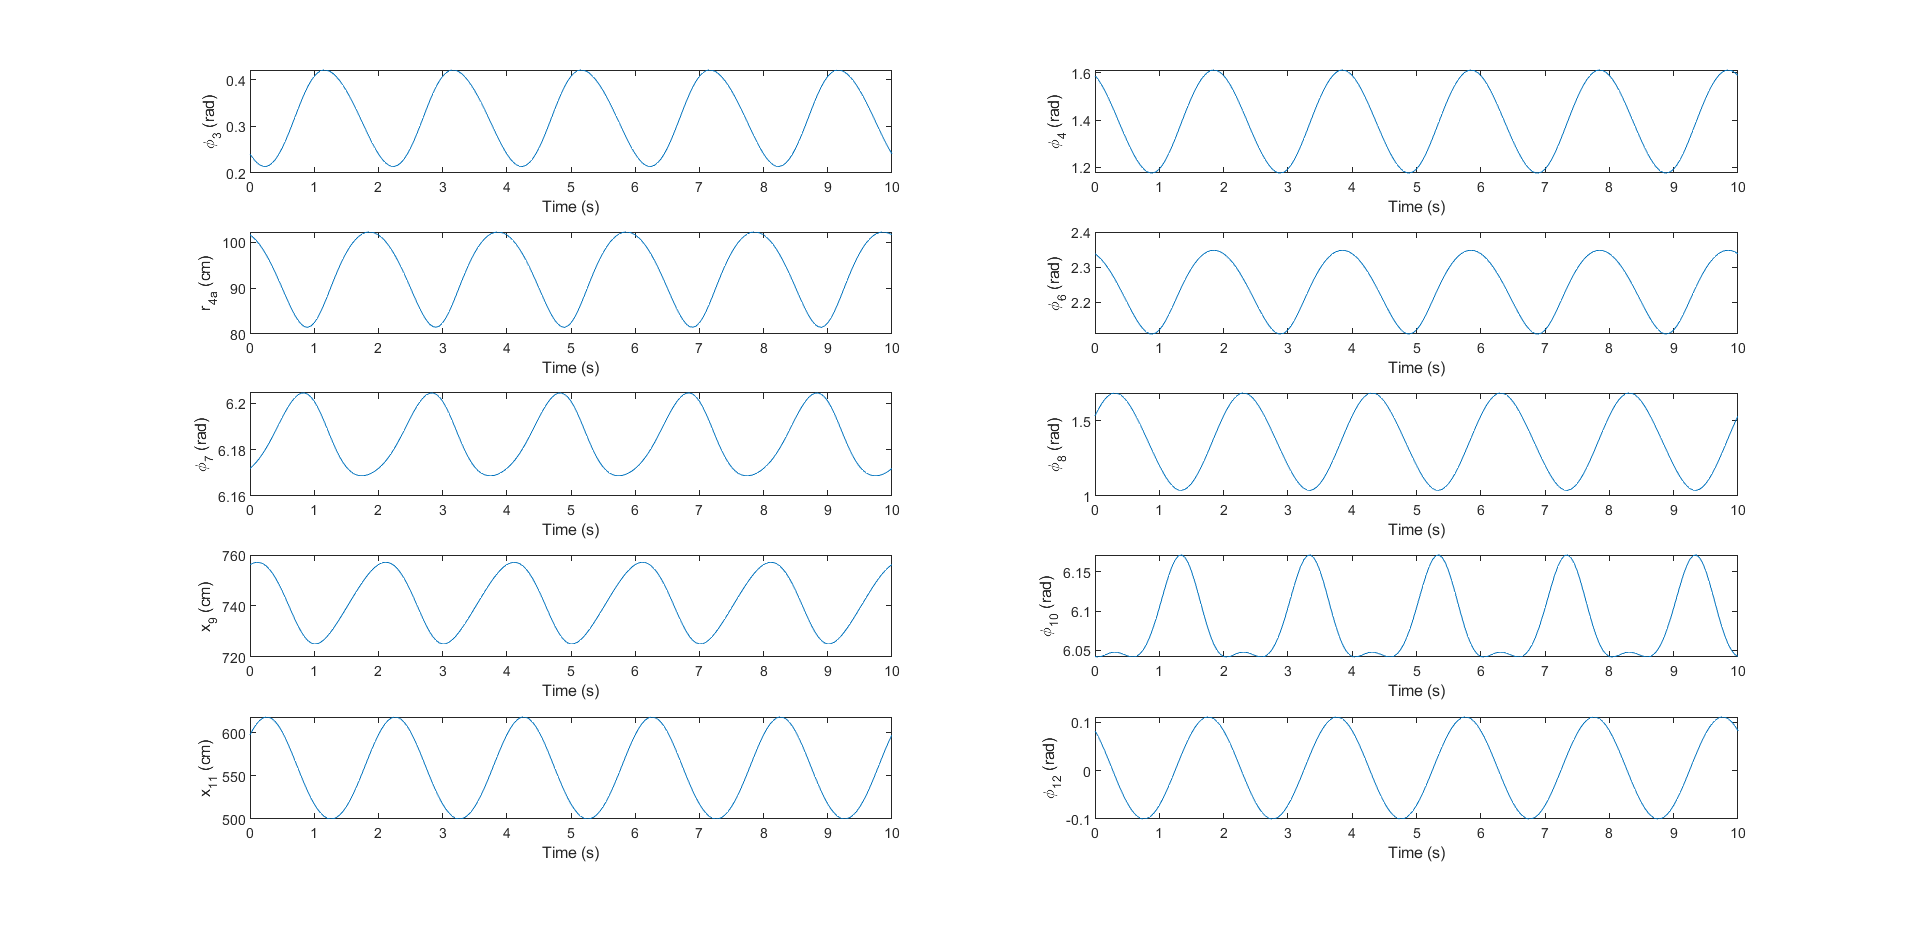
\includegraphics[width = \textwidth]{kinpos.png}
	
	\caption{Angles of the bodies (to the positive x axis), distance from joint (D) to (H) and x coordinates of the pistons (according to (A)) in function of time.}
	\label{fig:kinpos}
	
\end{figure}



\subsection{Velocity analysis}

The velocity analysis finds the ten unknown variables \(\diff{\phi_3(t)}{t}\), \(\diff{\phi_4(t)}{t}\), \(\diff{r_{4a}(t)}{t}\), \(\diff{\phi_6(t)}{t}\), \(\diff{\phi_7(t)}{t}\), \(\diff{\phi_8(t)}{t}\), \(\diff{x_9(t)}{t}\), \(\diff{\phi_{10}(t)}{t}\), \(\diff{x_{11}(t)}{t}\) and \(\diff{\phi_{12}(t)}{t}\).

The first order time derivatives of the loop closure equations~\ref{eq:loopclosurevec} are now used to find these unknown velocities. They are listed in the MATLAB function \texttt{velocity\char`_eqs.m}. The first order derivative of body (2) is known and is defined in equation~\ref{eq:dphi2}. 

The new set of loop closure equations is now linear because the derivative of the multiplication of \(\phi_4(t)\) and \(r_{4a}(t)\) contains no multiplication of the now unknown \(\diff{\phi_4(t)}{t}\) and \(\diff{r_{4a}(t)}{t}\).

The MATLAB code solves this system and returns values for the velocities of the bodies in function of the time. They are plotted in figure~\ref{fig:kinvel}.

\begin{figure}[h]
	\centering
	
	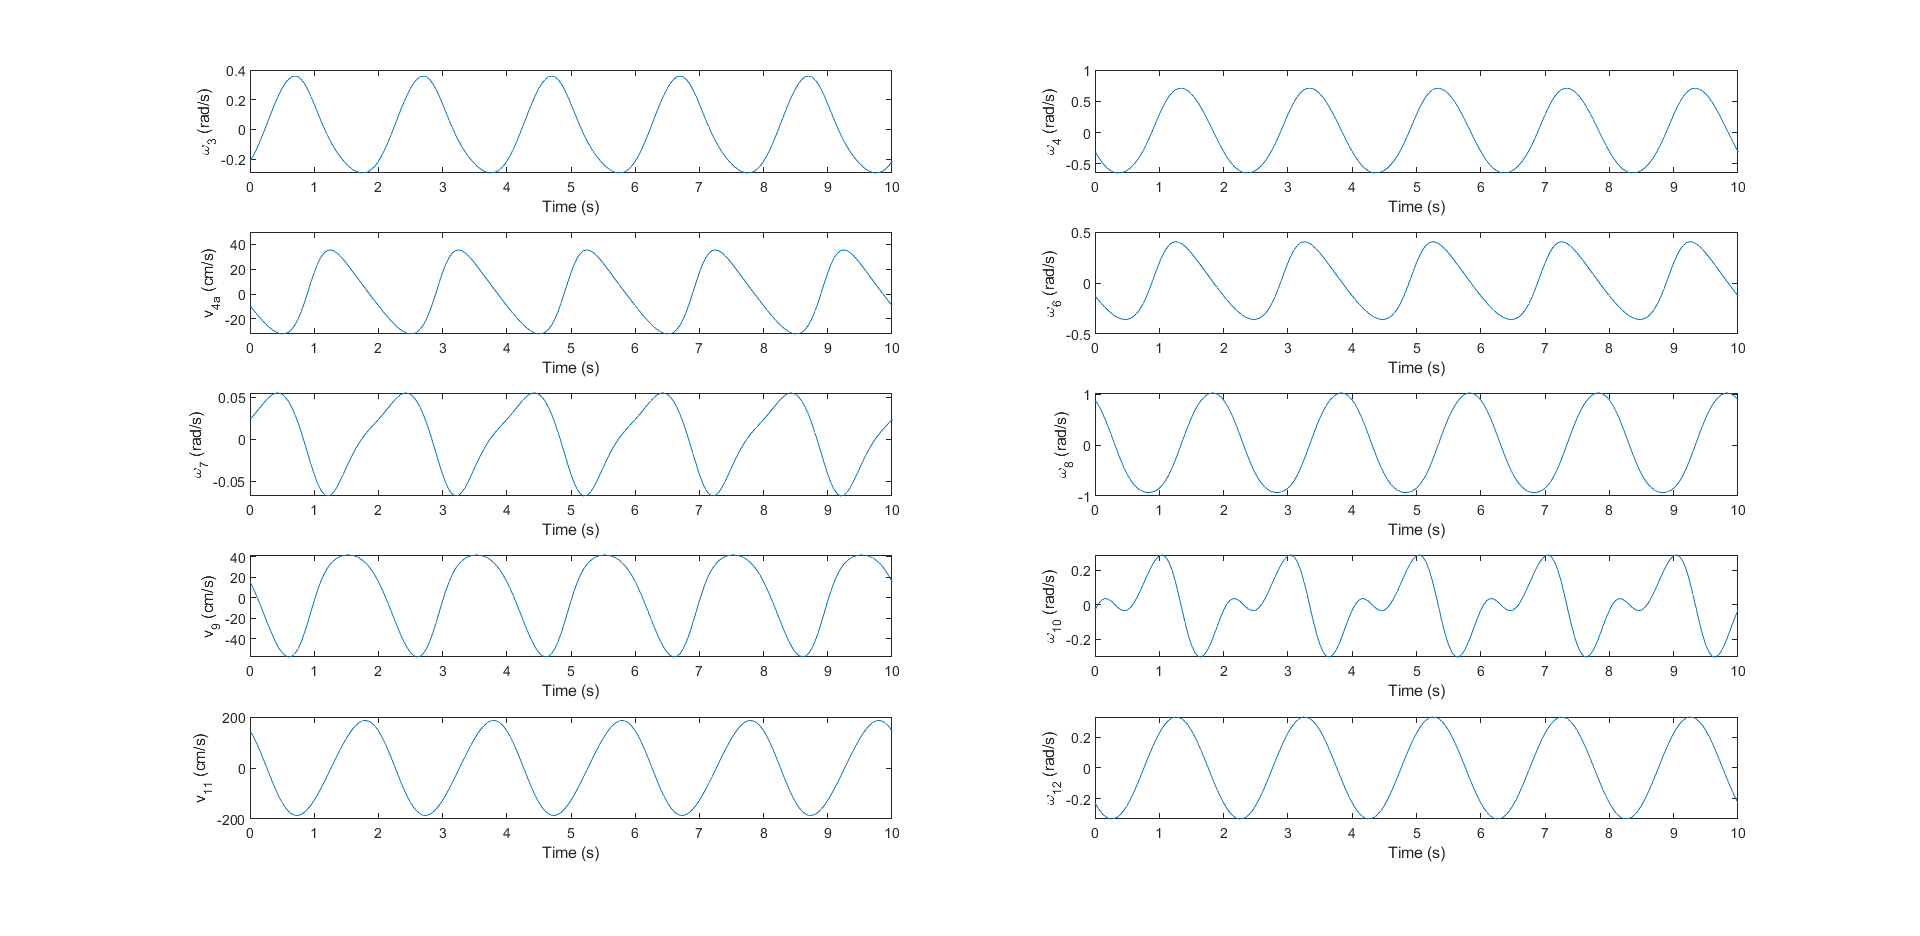
\includegraphics[width = \textwidth]{kinvel.png}
	
	\caption{Angular velocities of the bodies (to the positive x axis) and linear velocities of joint (H) (according to (D)) and of the pistons (according to (A)) in function of time.}
	\label{fig:kinvel}
	
\end{figure}

\newpage

\subsection{Acceleration analysis}

The acceleration analysis finds the ten unknown variables \(\diff[2]{\phi_3(t)}{t}\), \(\diff[2]{\phi_4(t)}{t}\), \(\diff[2]{r_{4a}(t)}{t}\), \(\diff[2]{\phi_6(t)}{t}\), \(\diff[2]{\phi_7(t)}{t}\), \(\diff[2]{\phi_8(t)}{t}\), \(\diff[2]{x_9(t)}{t}\), \(\diff[2]{\phi_{10}(t)}{t}\), \(\diff[2]{x_{11}(t)}{t}\) and \(\diff[2]{\phi_{12}(t)}{t}\).

This happens analogously to the velocity analysis. The MATLAB code now solves a linear set of the second order time derivatives of the ten loop closure equations. These are listed in the MATLAB function \texttt{acceleration\char`_eqs.m}. The plots of the accelerations of the bodies are shown in figure~\ref{fig:kinacc}.

\begin{figure}[h]
	\centering
	
	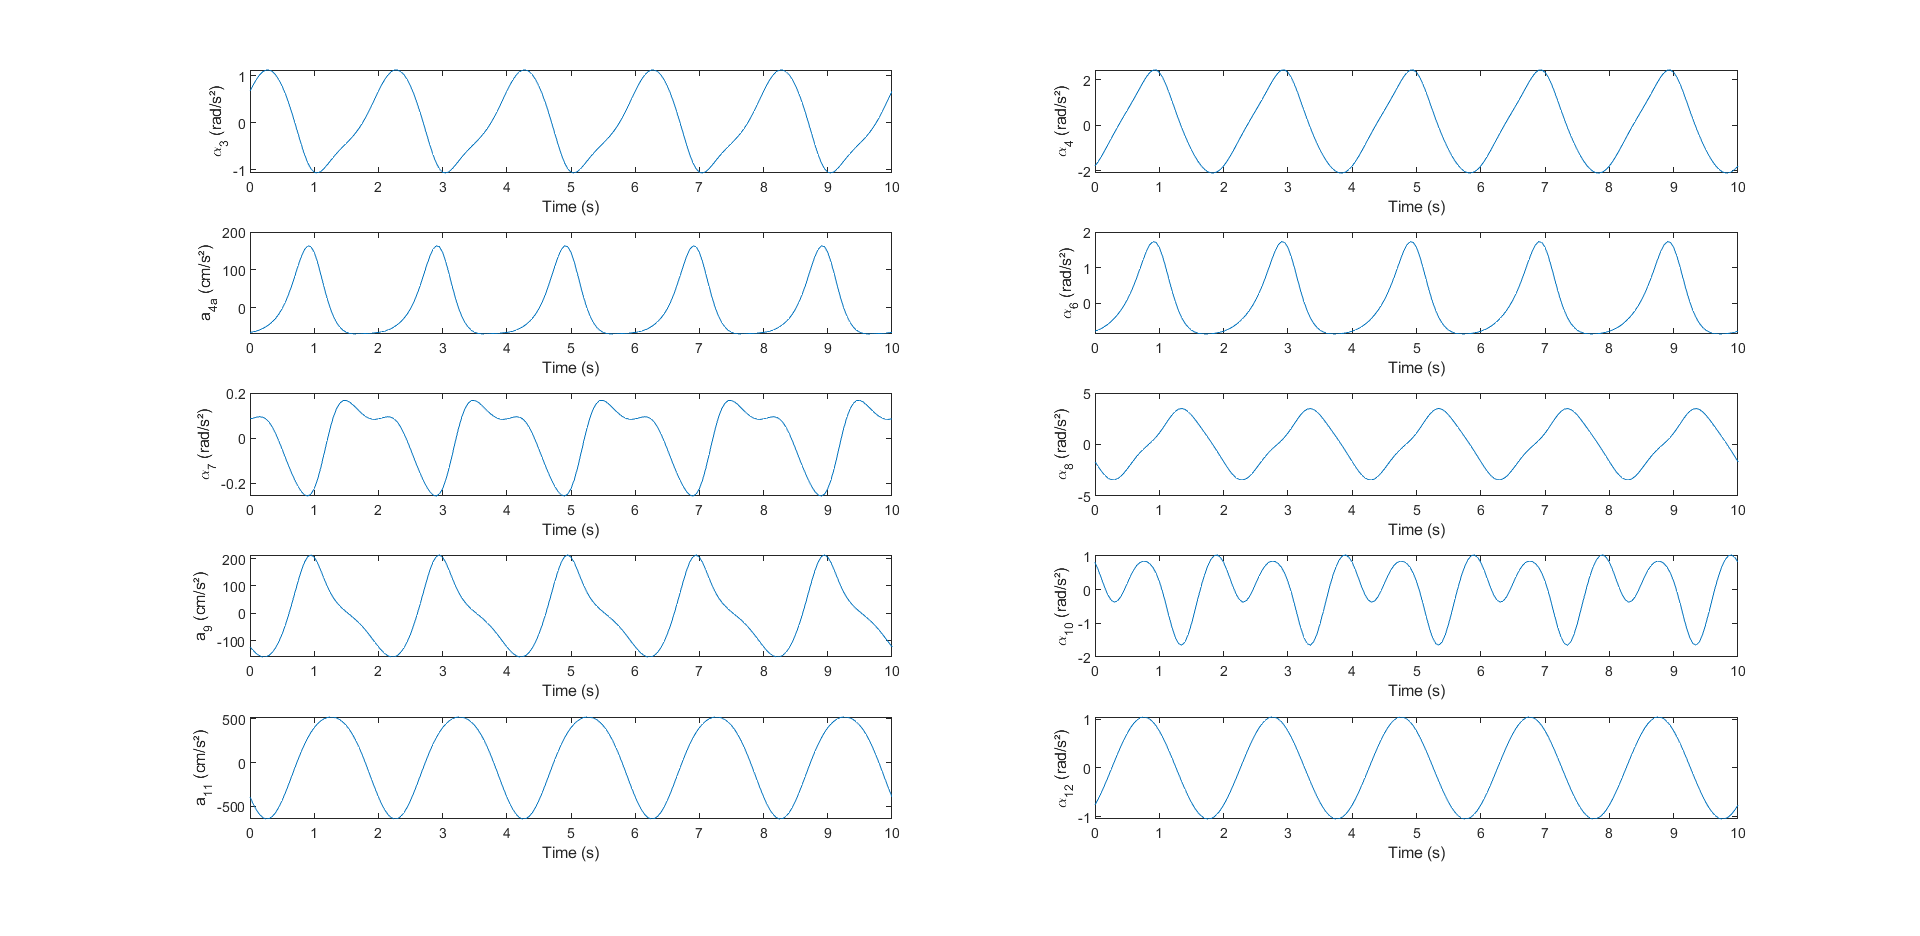
\includegraphics[width = \textwidth]{kinacc.png}
	
	\caption{Angular accelerations of the bodies (to the positive x axis) and linear accelerations of joint (H) (according to (D)) and of the pistons (according to (A)) in function of time.}
	\label{fig:kinacc}
	
\end{figure}


\subsection{Checking the results}

When writing the equations, there are places where errors can easily sneak in (e.g. notation errors). To check whether the generated results are correct, control calculations have been made. This section will be about checking the kinematics.

\subsubsection{Checking the position}

To check the position, we calculate the position of the joint (F) in two different ways. First, because (F) is a stationary point, it can be calculated via the given distance and angle to (A):

\begin{equation}
	\vec{F_1} = r_{1b}*e^{i*\phi_{AF}}
\end{equation}

The second way is by following a path of consecutive points in the mechanism from (A) to (F):

\begin{equation}
	\vec{F_2} = r_{2c}*e^{i*(\phi_2 + \phi_A)} + r_3*e^{i*\phi_3} + r_4*e^{i*\phi_4}
\end{equation}

The x and y components of these vectors can be found by taking respectively the real and imaginary part of these complex numbers. The difference between \(\vec{F_1}\) and \(\vec{F_2}\) is plotted in figure \ref{fig:contrpos}. The x and y components match well, there is nothing special to report there. 

The relative error \(1 – \vec{F_1}/\vec{F_2}\) takes on values of the order of \(10^{-12}\) cm and the absolute error \(\vec{F_1}-\vec{F_2}\) is of the order of \(10^{-10}\) cm. This is not yet near machine precision, so the error is probably a result of using \texttt{fsolve}. The error is small enough to consider this check successful.

We can also visually inspect the position results by watching an animation of the mechanism. In the animation in the attached MATLAB code \footnote{The animation pops up when running \texttt{main.m} with \texttt{movie\char`_12bar = 1;} on line 22 of the code.} one can see that point (F) (like (A) and (E)) doesn’t move.

\begin{figure}
	\centering
	
	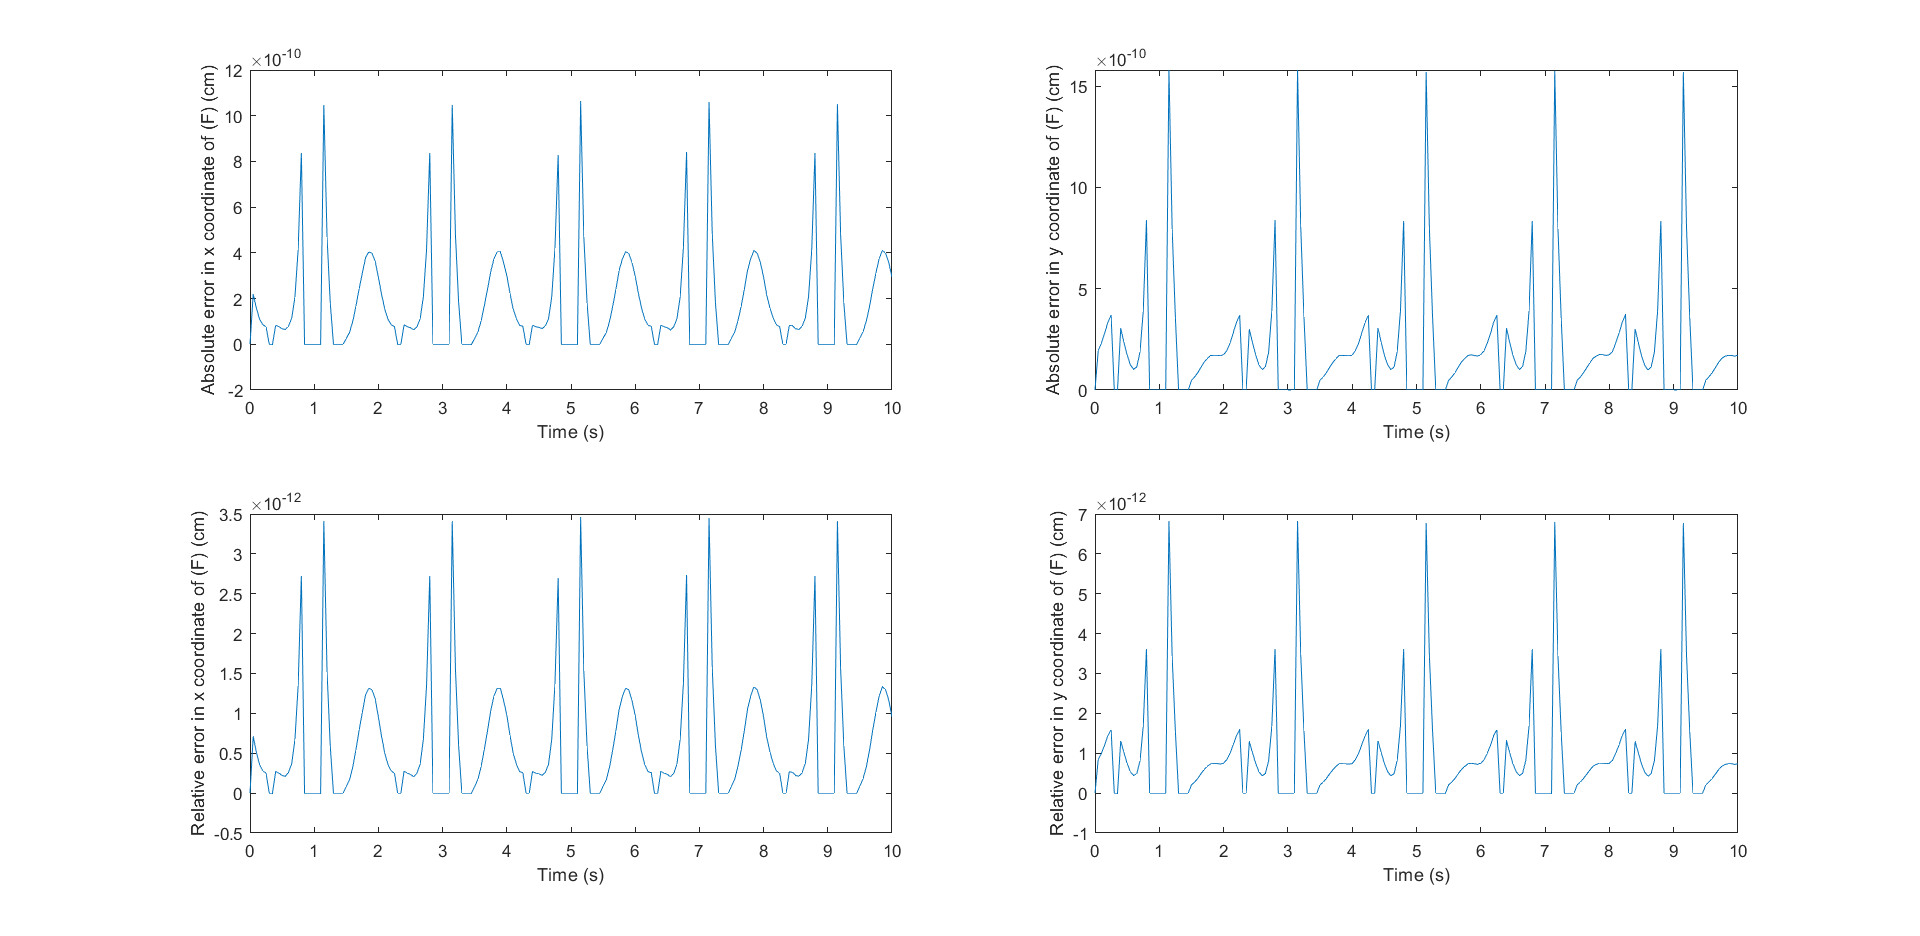
\includegraphics[width = \textwidth]{contrpos.png}
	
	\caption{Position errors in coordinates of point (F) in function of time.}
	\label{fig:contrpos}
	
\end{figure}

\subsubsection{Checking the velocity and the acceleration}

Checking the speed and acceleration is done in the same way. Because (F) is a stationary point, its velocity and acceleration have to be equal to zero at all times. This means that by plotting the velocity or acceleration of (F) calculated via a path of consecutive points from (A) to (F), one will plot the error.

The velocity of point (F) (via (A)) can be calculated as follows:

\begin{equation}
	\vec{v_F} = \vec{\omega_2}\times\vec{AC}+ \vec{\omega_3}\times\vec{CD}+ \vec{\omega_4}\times\vec{DF}
\end{equation}

Figure~\ref{fig:contrvel} presents the error in velocity of point (F). The x and y components match well, there is nothing special to report there. Except for the two deviating values, this error seems to stay perfectly at 0. After zooming in we can see that this error doesn’t perfectly equal 0 but is instead in the order of \(10^{-14}~\si{cm/s}\). This is starting to approach machine precision but is still not as precise. Again, the error is a result of using \texttt{fsolve}. The error is small enough to consider this check successful.

The acceleration of point (F) (via (A)) can be calculated as follows:

\begin{equation}
	\vec{a_F} = \vec{\omega_2}\times(\vec{\omega_2}\times\vec{AC}) + \vec{\alpha_2}\times\vec{AC} + \vec{\omega_3}\times(\vec{\omega_3}\times\vec{CD}) + \vec{\alpha_3}\times\vec{CD} + \vec{\omega_4}\times(\vec{\omega_4}\times\vec{DF}) + \vec{\alpha_4}\times\vec{DF}
\end{equation}

Figure~\ref{fig:contracc} shows the acceleration error. Once again the x and y components match so there is nothing special to report. The error here is from the order of \(10^{-14}~\si{cm/s^2}\). Like with the position and velocity errors, this isn’t machine precision yet, but a deviation introduced by \texttt{fsolve}. It is small enough to consider this check successful.

\begin{figure}
	\centering
	
	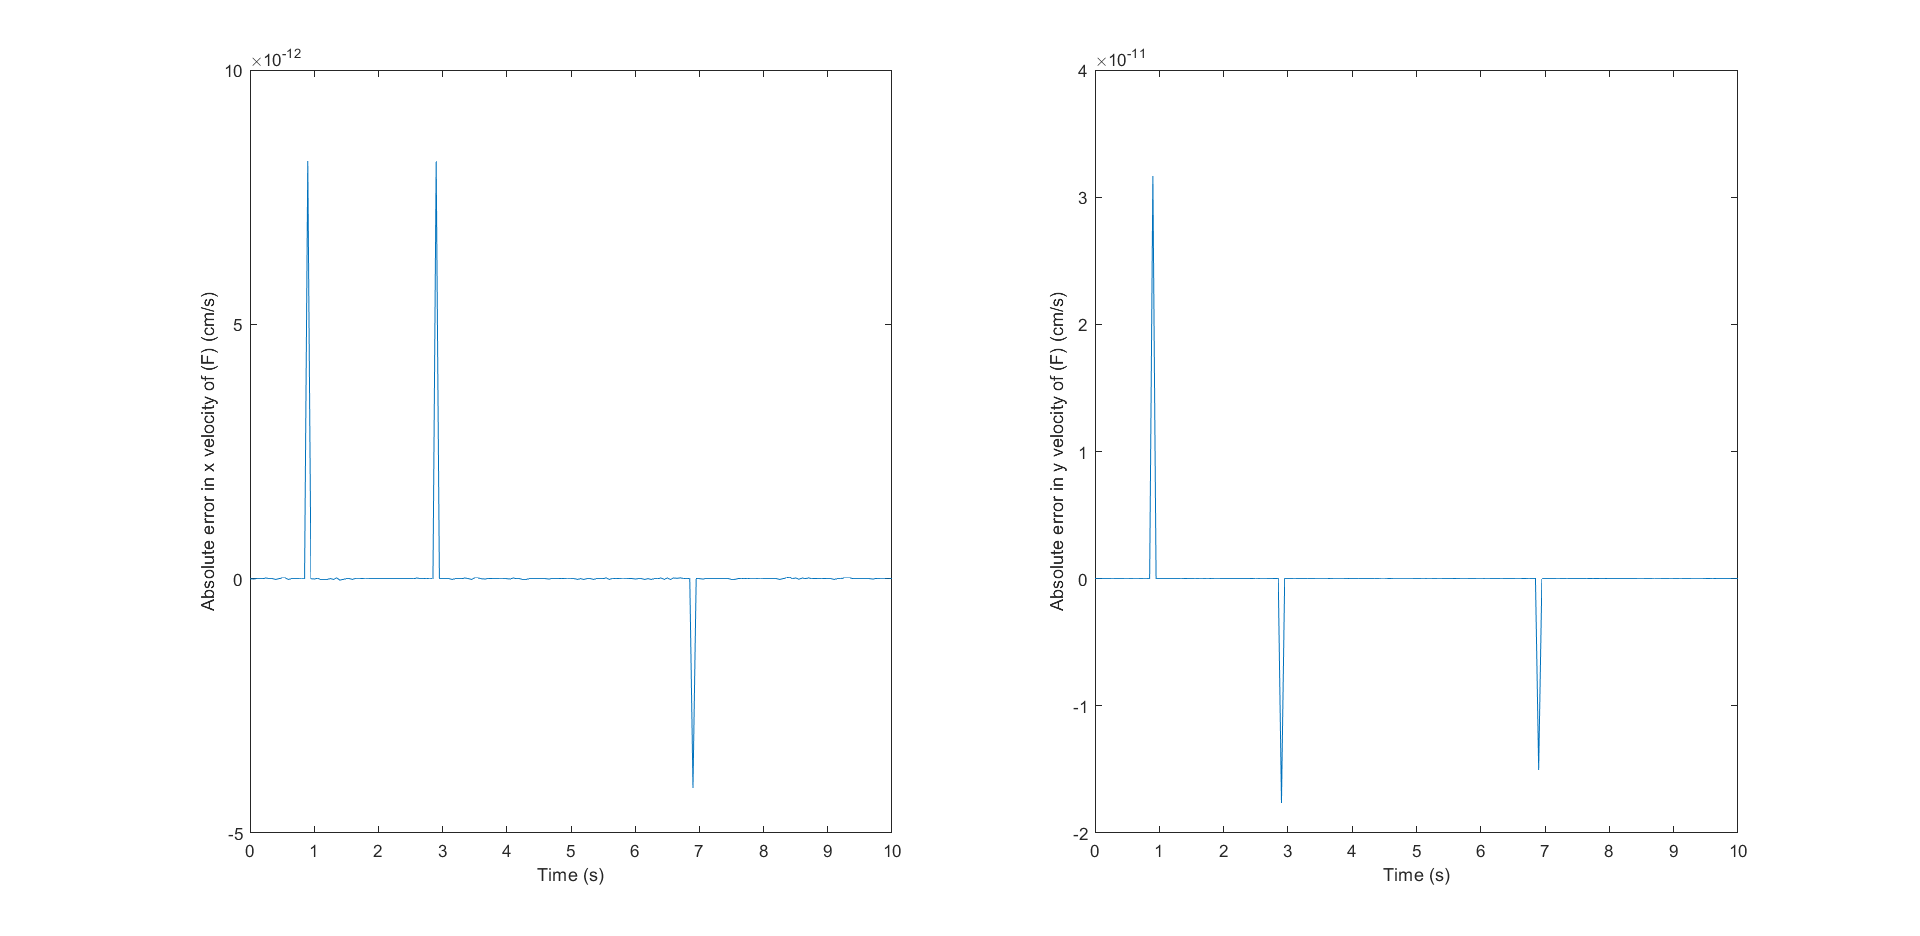
\includegraphics[width = \textwidth]{contrvel.png}
	
	\caption{Velocity errors in coordinates of point (F) in function of time.}
	\label{fig:contrvel}
	
\end{figure}

\begin{figure}
	\centering
	
	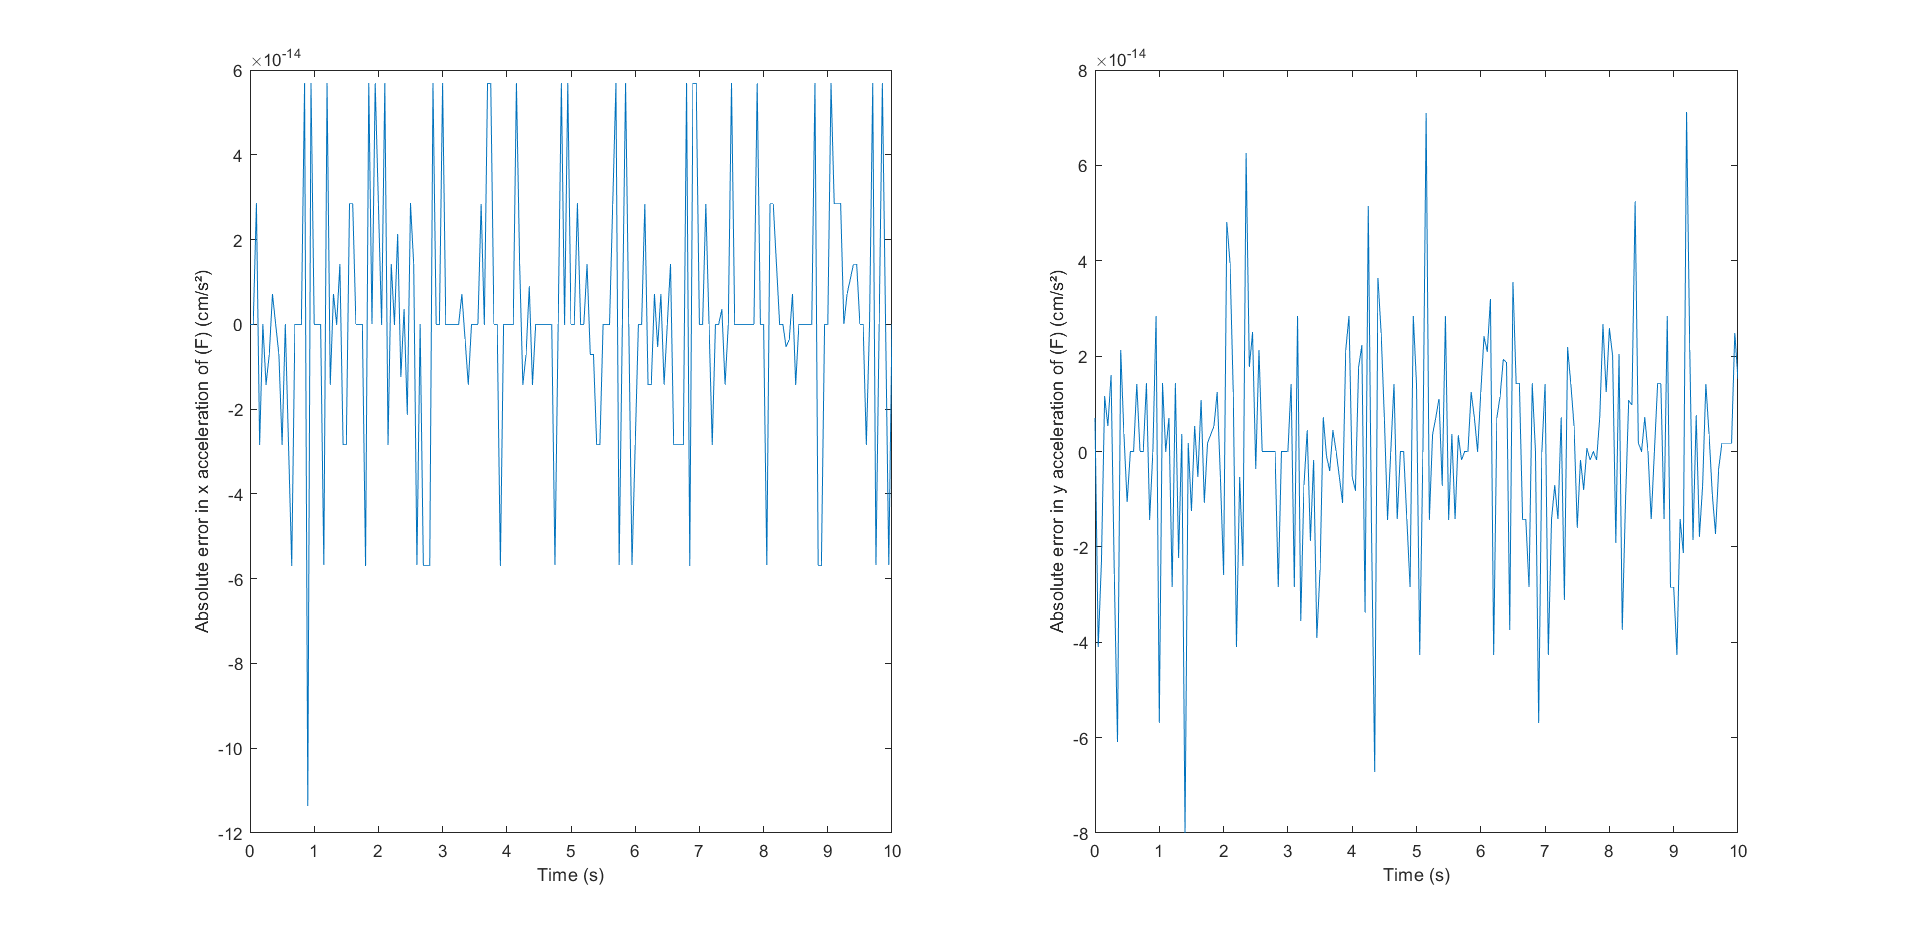
\includegraphics[width = \textwidth]{contracc.png}
	
	\caption{Acceleration errors in coordinates of point (F) in function of time.}
	\label{fig:contracc}
	
\end{figure}

\section{Dynamic analysis}

\subsection{Inverse dynamic analysis}

The dynamic analysis determines the 32 internal reaction forces or torques and the driving torque on the wheel. These forces and torques are defined in figure~\ref{fig:dyndef}.

\begin{figure}[h]
	\centering
	
	\includegraphics[width = .77\textwidth]{dyndef.jpg}
	
	\caption{Definition of the internal reactions forces and torques.}
	\label{fig:dyndef}
	
\end{figure}

In order to calculate these 33 unknown variables, a linear system of 33 equations is set up. Each of the eleven bodies (without the ground (1)) gives three dynamic equations: one for the forces in the x direction, one for the forces in the y direction and one for the torques around the z axis. The 33 equations can be found below:

\bigskip

Body (2):

\begin{subequations}
	\begin{equation}
		F_{A,x} + F_{B,x} + F_{C,x}=m_2*a_{2,x}
	\end{equation}
	\begin{equation}
		F_{A,y} + F_{B,y} + F_{C,y}=m_2*a_{2,y}
	\end{equation}
	\begin{equation}
	\begin{split}
		-F_{A,x}*|cog_2A|_y+F_{A,y}*|cog_2A|_x+M_{A,z}\\-F_{B,x}*|cog_2B|_y+F_{B,y}*|cog_2B|_x\\-F_{C,x}*|cog_2C|_y+F_{C,y}*|cog_2C|_x\\=I_2*\alpha_2
	\end{split}
	\end{equation}
\end{subequations}

Body (3):

\begin{subequations}
	\begin{equation}
		-F_{C,x} + F_{D,x}=m_3*a_{3,x}
	\end{equation}
	\begin{equation}
		-F_{C,y} + F_{D,y}=m_3*a_{3,y}
	\end{equation}
	\begin{equation}
	\begin{split}
		F_{C,x}*|cog_3C|_y-F_{C,y}*|cog_3C|_x\\-F_{D,x}*|cog_3D|_y+F_{D,y}*|cog_3D|_x\\=I_3*\alpha_3
		\end{split}
	\end{equation}
\end{subequations}


Body (4):

\begin{subequations}
	\begin{equation}
		-F_{D,x}+F_{F,x}-F_{I,n}*cos(\phi_4)=m_4*a_{4,x}
	\end{equation}
	\begin{equation}
		-F_{D,y}+F_{F,y}+F_{I,n}*sin(\phi_4)=m_4*a_{4,y}
	\end{equation}
	\begin{equation}
	\begin{split}
		F_{D,x}*|cog_4D|_y-F_{D,y}*|cog_4D|_x\\-F_{F,x}*|cog_4F|_y+F_{F,y}*|cog_4F|_x\\=I_4*\alpha_4
	\end{split}
	\end{equation}
\end{subequations}

Body (5):

\begin{subequations}
	\begin{equation}
		-F_{H,x}+F_{I,n}*cos(\phi_4)=m_5*a_{5,x}=0
	\end{equation}
	\begin{equation}
		-F_{H,y}-F_{I,n}*sin(\phi_4)=m_5*a_{5,y}=0
	\end{equation}
	\begin{equation}
		-M_{I,z}=I_5*\alpha_5=0
	\end{equation}
\end{subequations}

Body (6):

\begin{subequations}
	\begin{equation}
		F_{E,x}+F_{G,x}=m_6*a_{6,x}
	\end{equation}
	\begin{equation}
		F_{E,y}+F_{G,y}=m_6*a_{6,y}
	\end{equation}
	\begin{equation}
	\begin{split}
		-F_{E,x}*|cog_6E|_y+F_{E,y}*|cog_6E|_x\\-F_{G,x}*|cog_6G|_y+F_{G,y}*|cog_6G|_x\\=I_6*\alpha_6
	\end{split}
	\end{equation}
\end{subequations}

Body (7):

\begin{subequations}
	\begin{equation}
		-F_{G,x}+F_{H,x}+F_{J,x}=m_7*a_{7,x}
	\end{equation}
	\begin{equation}
		-F_{G,y}+F_{H,y}+F_{J,y}=m_7*a_{7,y}
	\end{equation}
	\begin{equation}
	\begin{split}
		F_{G,x}*|cog_7G|_y-F_{G,y}*|cog_7G|_x\\-F_{H,x}*|cog_7H|_y+F_{H,y}*|cog_7H|_x\\-F_{J,x}*|cog_7J|_y+F_{J,y}*|cog_7J|_x\\=I_7*\alpha_7
		\end{split}
	\end{equation}
\end{subequations}

Body (8):

\begin{subequations}
	\begin{equation}
		-F_{J,x}+F_{K,x}+F_{M,x}=m_8*a_{8,x}
	\end{equation}
	\begin{equation}
		-F_{J,y}+F_{K,y}+F_{M,y}=m_8*a_{8,y}
	\end{equation}
	\begin{equation}
	\begin{split}
	F_{J,x}*|cog_8J|_y-F_{J,y}*|cog_8J|_x\\-F_{K,x}*|cog_8K|_y+F_{K,y}*|cog_8K|_x\\-F_{M,x}*|cog_8M|_y+F_{M,y}*|cog_8M|_x\\=I_8*\alpha_8
	\end{split}
	\end{equation}
\end{subequations}

Body (9):

\begin{subequations}
	\begin{equation}
		-F_{K,x}=m_9*a_{9,x}
	\end{equation}
	\begin{equation}
		-F_{K,y}+F_{L,y}=m_9*a_{9,y}
	\end{equation}
	\begin{equation}
	\begin{split}
	F_{K,x}*|cog_{9}K|_y-F_{K,y}*|cog_{9}K|_x\\+F_{L,y}*|cog_{9}L|_x+M_{L,z}\\=I_{9}*\alpha_{9}
	\end{split}
	\end{equation}
\end{subequations}

Body (10):

\begin{subequations}
	\begin{equation}
		-F_{M,x}-F_{O,x}=m_{10}*a_{10,x}
	\end{equation}
	\begin{equation}
		-F_{M,y}-F_{O,y}=m_{10}*a_{10,y}
	\end{equation}
	\begin{equation}
	\begin{split}
	F_{M,x}*|cog_{10}M|_y-F_{M,y}*|cog_{10}M|_x\\F_{O,x}*|cog_{10}O|_y-F_{O,y}*|cog_{10}O|_x\\=I_{10}*\alpha_{10}
	\end{split}
	\end{equation}
\end{subequations}

Body (11):

\begin{subequations}
	\begin{equation}
		-F_{N,x}+F_{O,x}=m_{11}*a_{11,x}
	\end{equation}
	\begin{equation}
		-F_{N,y}+F_{O,y}+F_{P,y}=m_{11}*a_{11,y}
	\end{equation}
	\begin{equation}
	\begin{split}
	F_{N,x}*|cog_{11}N|_y-F_{N,y}*|cog_{11}N|_x\\-F_{O,x}*|cog_{11}O|_y+F_{O,y}*|cog_{11}O|_x\\+F_{P,y}*|cog_{11}P|_x+M_{P,z}\\=I_{11}*\alpha_{11}
	\end{split}
	\end{equation}
\end{subequations}

Body (12):

\begin{subequations}
	\begin{equation}
		-F_{B,x}+F_{N,x}=m_{12}*a_{12,x}
	\end{equation}
	\begin{equation}
		-F_{B,y}+F_{N,y}=m_{12}*a_{12,y}
	\end{equation}
	\begin{equation}
	\begin{split}
	F_{B,x}*|cog_{12}B|_y-F_{B,y}*|cog_{12}B|_x\\-F_{N,x}*|cog_{12}N|_y+F_{N,y}*|cog_{12}N|_x\\=I_{12}*\alpha_{12}
	\end{split}
	\end{equation}
\end{subequations}

The masses of the bodies are \(m_i=V_i*\rho_{steel}\) with \(\rho_{steel}=7800~\si{kg/m^3}\) \cite{steel1}. The linear accelerations of the bars are calculated by multiplicating the angular accelerations with the distance from the joint to the center of gravity of the bar. All these equations are implemented in the MATLAB function \texttt{dynamics\char`_12bar.m}.

\begin{figure}[h]
	\centering
	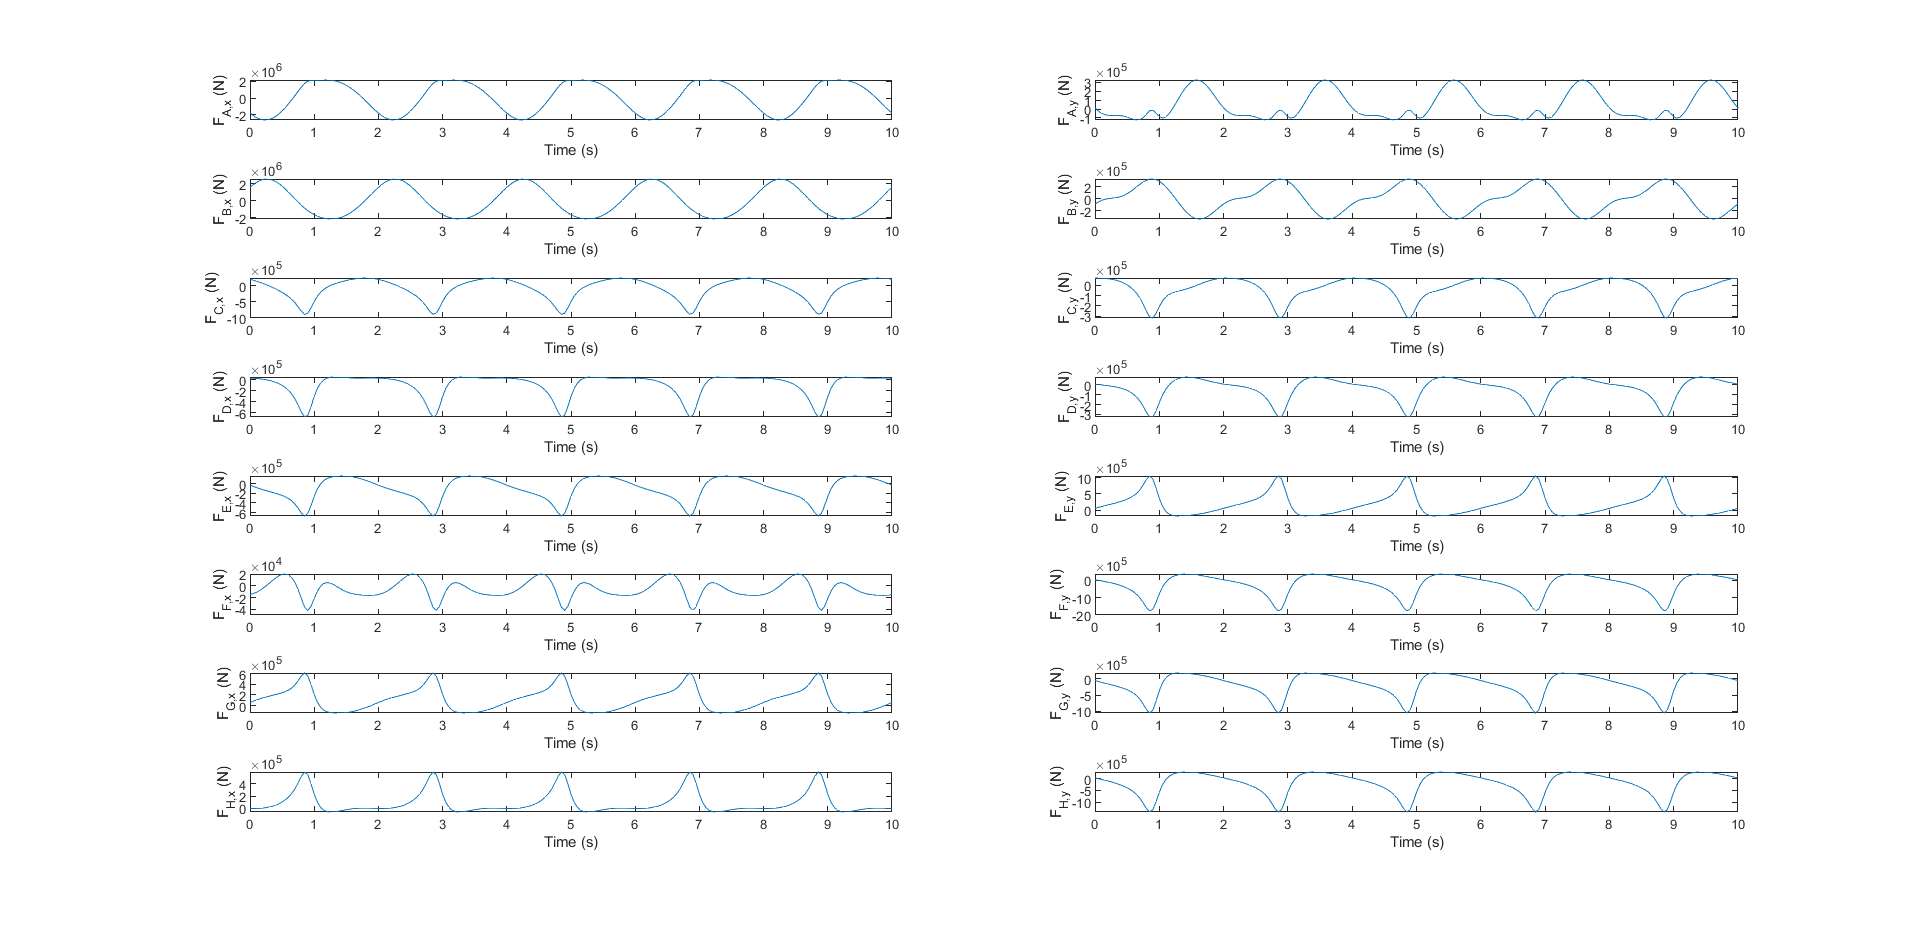
\includegraphics[width = .9\textwidth]{dynplot1.png}
	
	\caption{Internal reaction forces and torques in function of time (Part 1/2).}
	\label{fig:dynplot1}
	
\end{figure}

\begin{figure}[h]
	\centering
	
	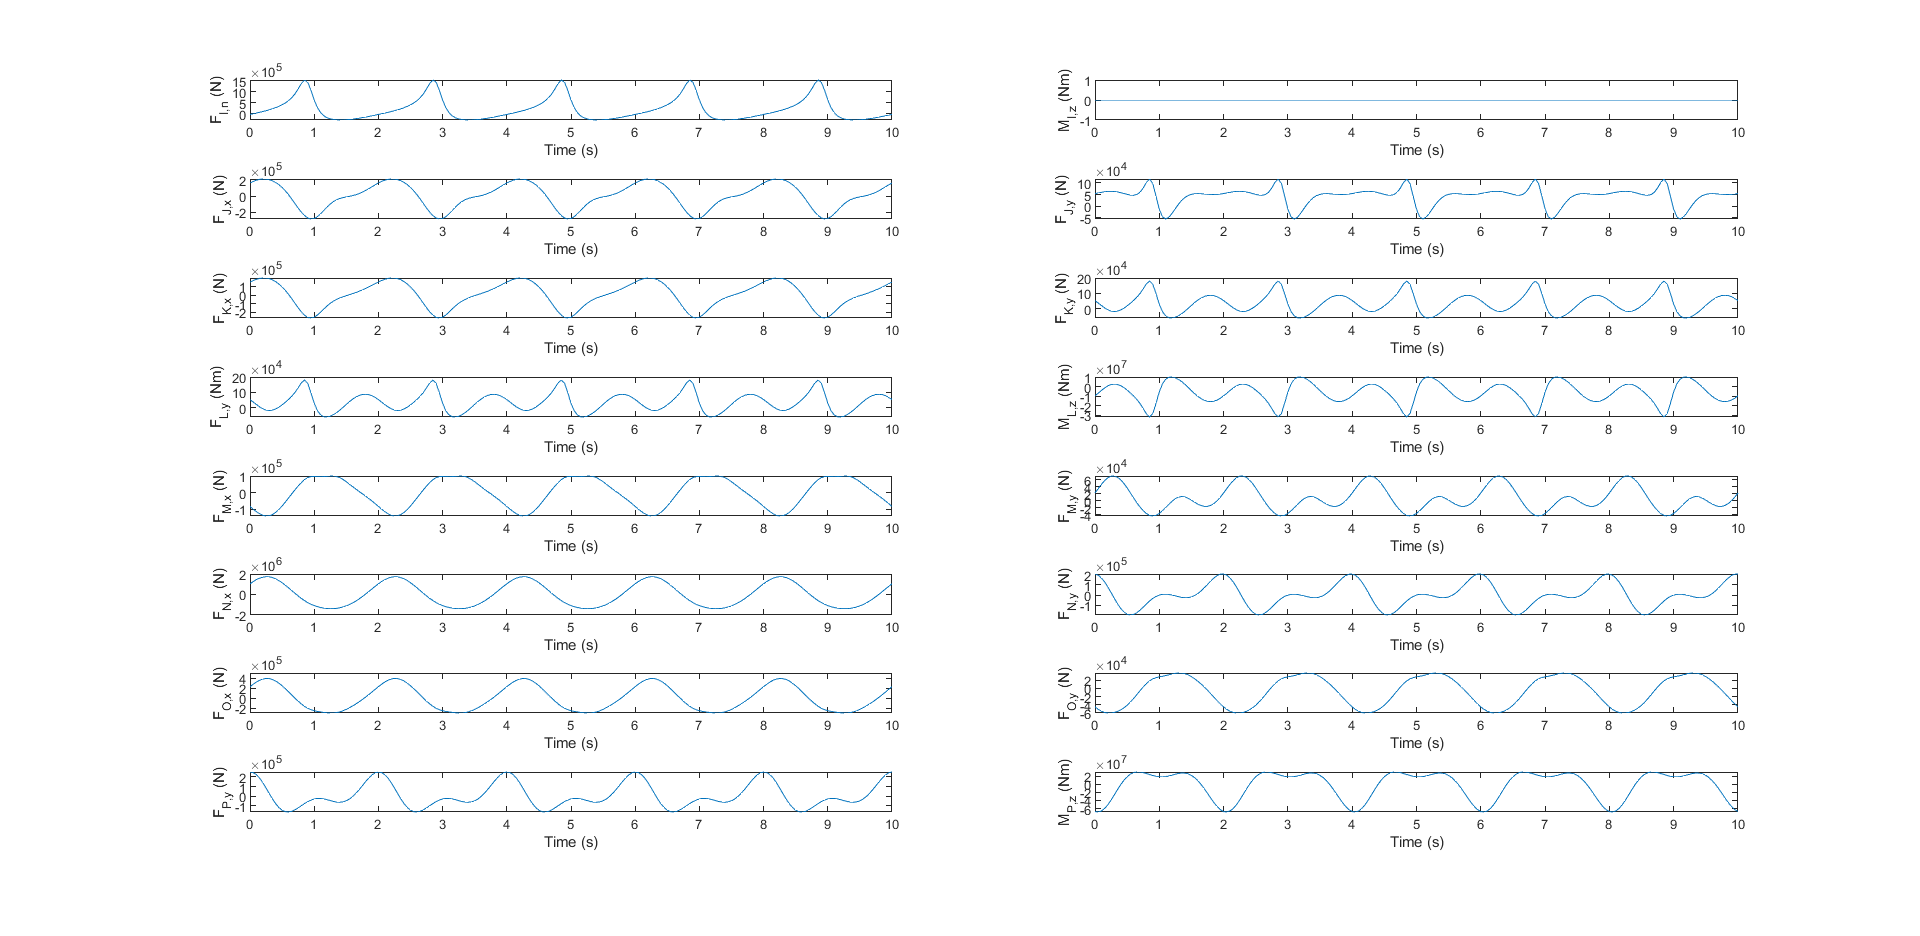
\includegraphics[width = .9\textwidth]{dynplot2.png}
	
	\caption{Internal reaction forces and torques in function of time (Part 2/2).}
	\label{fig:dynplot2}
	
\end{figure}

After solving this linear set of equations, the MATLAB code returns values for the 33 forces and torques for each time sample. The plots of these forces and torques in function of the time are listed in figures~\ref{fig:dynplot1},~\ref{fig:dynplot2} and~\ref{fig:dynplot3}.

\begin{figure}[h]
	\centering
	
	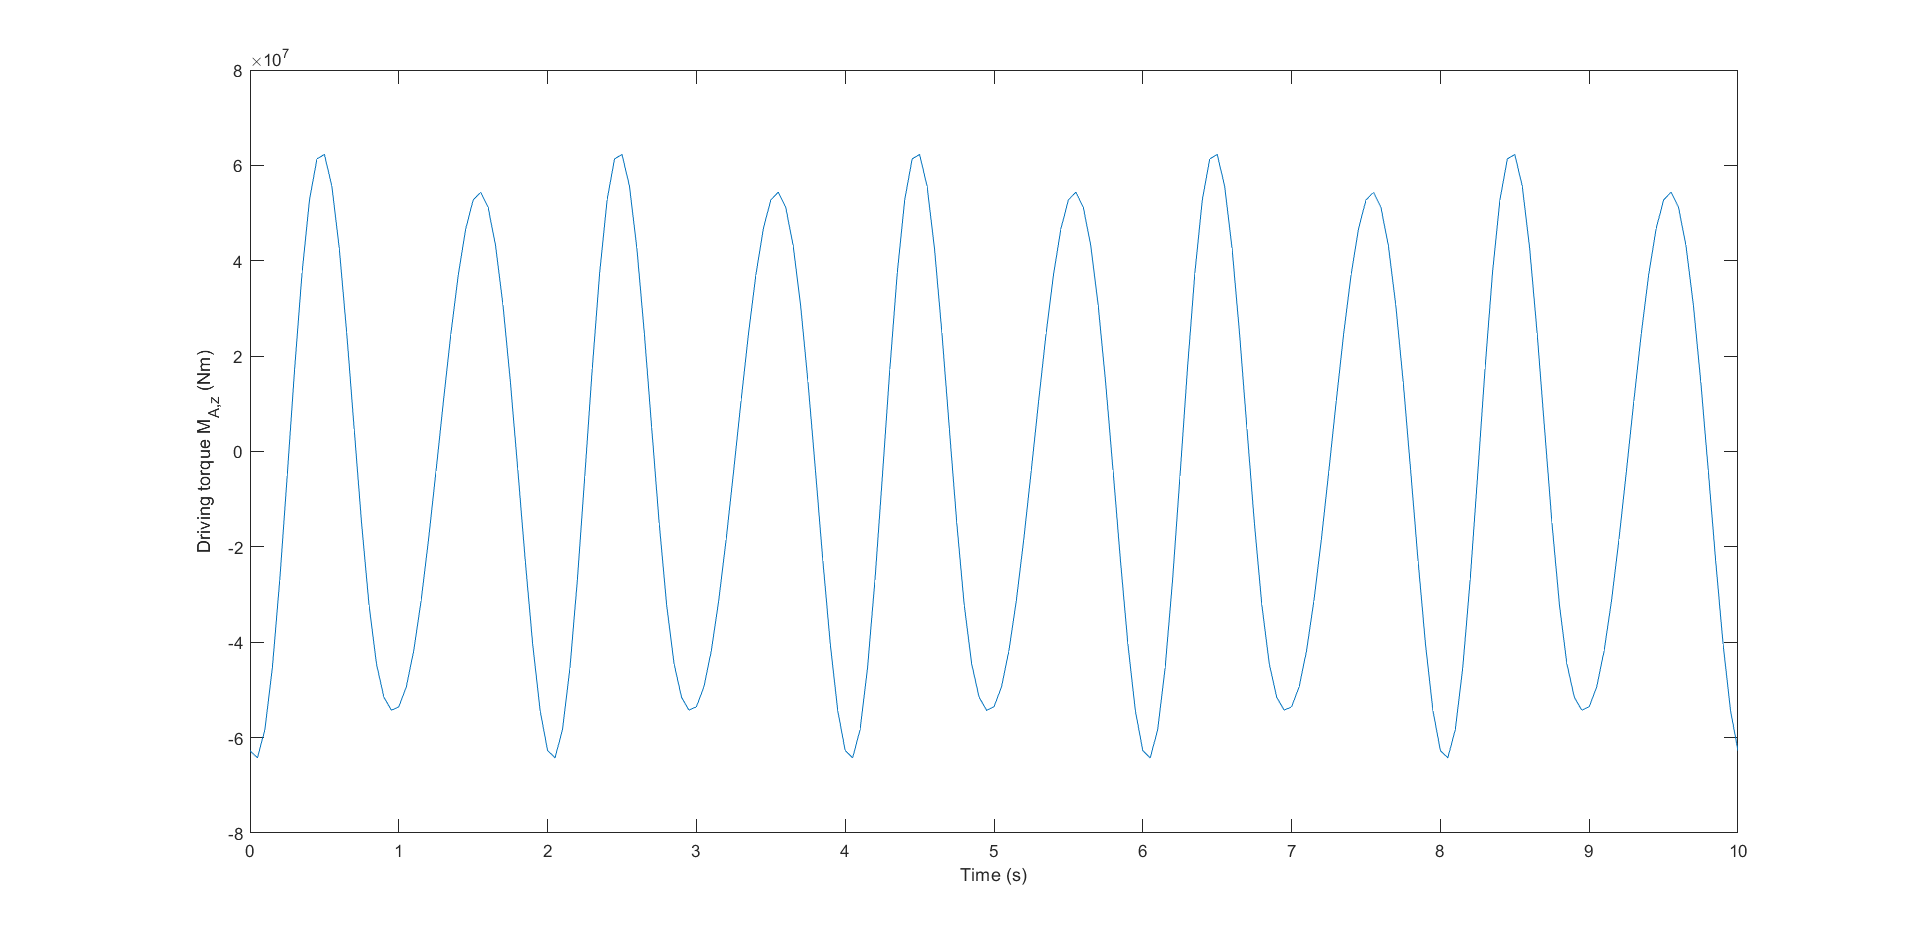
\includegraphics[width = \textwidth]{dynplot3.png}
	
	\caption{Driving torque in function of time.}
	\label{fig:dynplot3}
	
\end{figure}

\subsection{Checking the results}

For checking the dynamics we make use of the method of shaking forces, in which we determine the reaction forces that act on the ground. These reaction forces are the opposites of the internal forces \(F_A\), \(F_F\) and \(F_E\) . The shaking forces are equal to these reaction forces on the ground: 

\begin{equation}
	F_{shake,x,1} = F_{A,x} + F_{F,x} + F_{E,x}
\end{equation}

and can also be calculated as follows (for the x components):

\begin{equation}
\begin{split}
	F_{shake,x,2} =  a_{2,x}*m_2 + a_{3,x}*m_3 + a_{4,x}*m_4 + a_{5,x}*m_5 \\ 
	 +a_{6,x}*m_6	+ a_{7,x}*m_7 + a_{8,x}*m_8 + a_{9,x}*m_9 \\
	 + a_{10,x}*m_{10} + a_{11,x}*m_{11} + a_{12,x}*m_{12}
\end{split}
\end{equation}

The y components are calculated analogously.

We make the sum over all linkages except for the ground. The error of the shaking forces \(F_{shake,x,1}-F_{shake,x,2}\) is plotted in  figure \ref{fig:contrdyn}. The x and y components match well enough, even though one is one order of magnitude greater than the other. The error is from the order of \(10^{-9}\) Newton for the x component and \(10^{-10}\) Newton for the y component. This error is greater than machine precision, but this is a result of the used math algorithm. The error is small enough to consider this check successful.

\clearpage

\begin{figure}
	\centering
	
	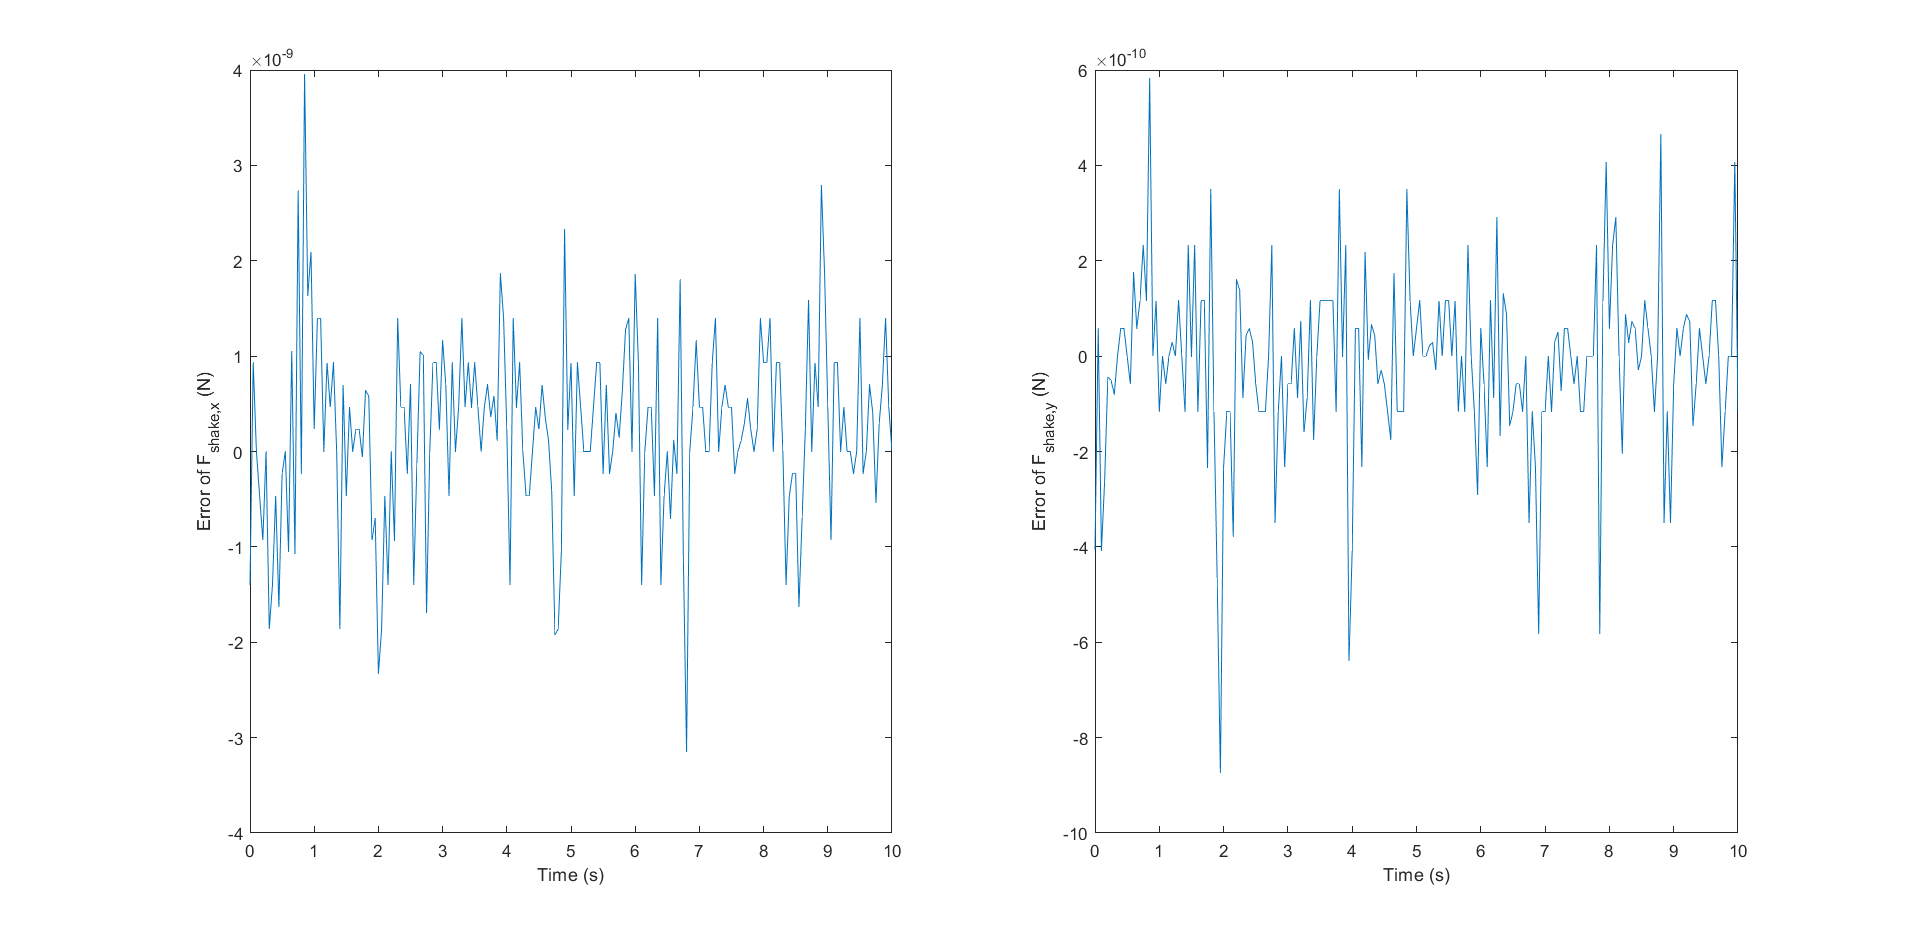
\includegraphics[width = \textwidth]{contrdyn.png}
	
	\caption{Error of the shaking forces in function of time.}
	\label{fig:contrdyn}
	
\end{figure}

\section*{Conclusion}

This report discusses a kinematic and dynamic analysis of a 12 bar linkage. Both the kinematic and dynamic analysis are very accurate. The errors of the results took on very small values that approach the machine accuracy. These results are clearly precise enough for eventual practical applications.

\bibliographystyle{plain}
\bibliography{walschaerts}


\end{document}